\section{Choix des algorithmes de traitement}
\label{sec:algo_trait}
Dans cette partie, l'objectif est de faire le choix des algorithmes qui seront utilisés dans ce projet. Les algorithmes considérés sont ceux présentés dans la partie [ref]. Elle débutera par la justification du choix de l'algorithme de formation d'images puis par celui de correction d'erreurs de phase.

\subsection{Algorithme de formation d'image}
\label{subsec:choix_bp}

Pour effectuer ce choix, le premier critère pris en compte est le mouvement du porteur. En effet, notre porteur est destiné à être un drone, relativement léger et donc sujet à d’importants écarts de trajectoire [à déterminer dans le cahier des charges]. Le premier critère est donc l’absence d’hypothèse de trajectoire linéaire dans les algorithmes. Dans ce cas, seul l’algorithme de \textit{Backprojection} respecte cette condition. Toutefois, pour nuancer ces propos, l’algorithme RMA permet une assez bonne correction de la trajectoire grâce à l’interpolation. Mais là encore, l’intégration de chaque contribution de chaque pixel dans l’algorithme de \textit{Backprojection} le rend plus robuste aux erreurs de phase. \
Un autre argument en faveur du RMA pourrait être sa complexité, bien moindre : $O(N^2 \log(N))$ contre $O(N^3)$ pour le \textit{Backprojection}. Cependant, dans ce projet, le traitement des données est réalisé post-mission, et aucune contrainte d’embarqué n’est donc considérée. \
Pour ces différentes raisons, nous faisons le choix d’utiliser l’algorithme de \textit{Backprojection} pour la formation d’image SAR.

\subsection{Algorithme de correction d'erreur de phase}
\label{subsec:choix_pga}

Pour l'implémentation de la correction d'erreur de phase, l'algorithme \textit{Phase Gradient Autofocus} (PGA) a été retenu. Cet algorithme est particulièrement robuste car il ne repose pas sur un modèle polynomial de l'erreur, permettant ainsi de corriger des distorsions de phase de fréquences élevées. Le détail de sa résolution est présenté ci-après.

L'objectif du PGA est d'estimer et de compenser le terme d'erreur de phase $\xi(x)$. La phase totale d'un signal reçu est cependant composite ; il est donc nécessaire d'isoler les termes d'intérêt en éliminant les composantes dites « parasites ». 

Dans la suite, nous distinguerons le \textbf{plan image} (données focalisées en pixels) du \textbf{plan signal} (données brutes après compression en distance, mais avant compression azimutale complète).

On définit l'expression de la phase du signal d'un pixel dans le plan image par :
\begin{equation}
\label{eq:phase}
    \Phi(x, y) \approx \frac{4 \pi}{\lambda} \left( R(x, y) + \xi(x) + \varphi(x, y) \right) 
\end{equation}
Où : 
\begin{itemize}
    \item $R(x, y)$ est la distance géométrique entre le capteur et la cible.
    \item $\xi(x)$ est l'erreur de phase induite par les défauts de trajectoire (que l'on cherche à estimer). 
    \item $\varphi(x, y)$ est la réponse de phase intrinsèque du diffuseur à la position $(x, y)$. 
\end{itemize}

En développant la distance $R(x, y) = \sqrt{R(y)^2 + (vt - x_0)^2}$ (où $v$ est la vitesse du porteur et $x_0$ la position de la cible) par une approximation paraxiale ($R(y) \gg x$), on obtient :
\begin{equation}
    \Phi(x, y) \approx \frac{4 \pi}{\lambda} \left( R(y) + \frac{(x - x_0)^2}{2R(y)} + \xi(x) + \varphi(x, y) \right)
\end{equation}

En considérant que le terme en $\frac{x^2}{2R(y)}$ est compensé lors de la formation de l'image, l'expression devient :
\begin{equation}
    \Phi(x, y) \approx \frac{4 \pi}{\lambda} \left( \underbrace{R(y) + \frac{x_0^2}{2R(y)} + \varphi(x, y)}_{\text{Termes constants}} - \frac{x \cdot x_0}{R(y)} + \xi(x) \right) 
\end{equation}

On observe un ensemble de termes constants sur l'axe azimutal pour une case de distance (\textit{range bin}) donnée. Pour les éliminer, l'algorithme estime le gradient de la phase. Toutefois, le terme $-\frac{x \cdot x_0}{R(y)}$, dépendant de l'azimut, subsisterait après dérivation (dépendance Doppler liée à l'excentricité de la cible).

Pour annuler ce terme, on réalise une étape de \textit{circular shifting} : pour chaque ligne (range bin), on identifie le diffuseur le plus brillant (\textit{dominant scatterer}) et on effectue une translation circulaire pour le centrer au milieu de l'image. Cela ramène $x_0$ à $0$, éliminant ainsi la rampe de phase linéaire. \cite{303752}

\begin{figure}[htbp]
    \centering
    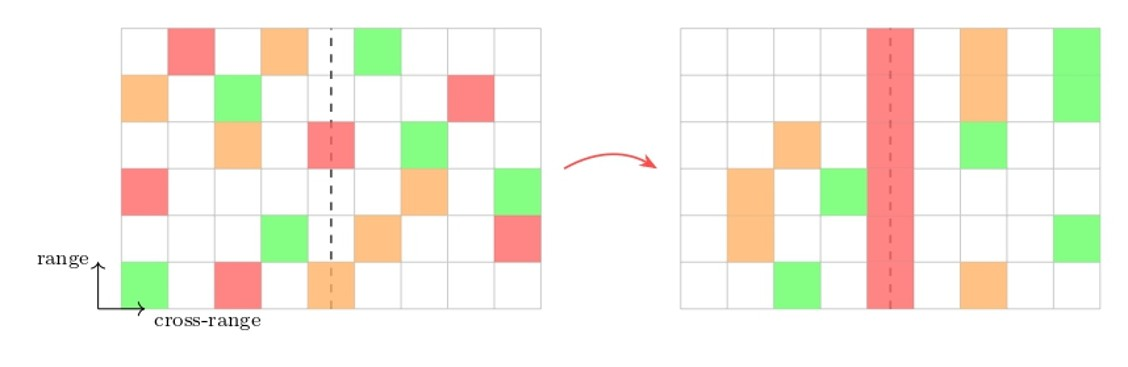
\includegraphics[width=0.7\linewidth]{src/rapport_complet/img/circ_shift.jpg}
    \caption{Principe du décalage circulaire (\textit{circular shifting}) pour le centrage des diffuseurs.}
    \label{fig:circshift}
\end{figure}

Ensuite, un fenêtrage est appliqué sur l'axe azimutal pour augmenter le SNR. Le signal fenêtré $s_c$ s'écrit :
\begin{equation}
    s_c(x - x_0, y) = \Pi_W(x) \cdot A(x - x_0, y) e^{-j \Phi(x - x_0, y)}
\end{equation}
Où $\Pi_W(x)$ est une fonction porte de largeur $W$. Cette largeur est réduite de manière itérative : plus l'image gagne en focalisation, plus la fenêtre est resserrée pour isoler le lobe principal du diffuseur.

Le passage dans le domaine fréquentiel azimutal permet alors d'isoler l'erreur de phase :
\begin{equation}
    s_c(x-x_0, y) \xrightarrow{\mathcal{F}_{az}} S_c(\eta, u) e^{-j2\pi x_0 u}
\end{equation}

L'estimation du gradient de la phase $\dot{\Phi}$ est réalisée par un estimateur de maximum de vraisemblance sur l'ensemble des $N$ \textit{range bins} \cite{303752} :
\begin{equation}
    \hat{\dot{\Phi}}(u) = \frac{\sum_{\eta=1}^{N} \Im\{S_c^*(\eta, u) \cdot \dot{S}_c(\eta, u)\}}{\sum_{\eta=1}^{N} |S_c(\eta, u)|^2} 
\end{equation}

Le résultat est ensuite intégré pour obtenir l'estimée de l'erreur $\hat{\xi}$, puis appliqué en correction. Le processus itère jusqu'à ce que la variation de l'erreur de phase soit inférieure à un seuil prédéfini. La structure globale est résumée en Figure \ref{fig:pga_custom}.
\begin{figure}[htbp]
    \centering
    \begin{tikzpicture}[node distance=1.3cm, font=\small, >=stealth, thick]
        % --- COLONNE 1 (Traitement Image) ---
        \node (start) [draw, rounded corners, fill=gray!10, text width=2.5cm, align=center] {Image SAR initiale};
        \node (shift) [draw, below of=start, fill=blue!15, text width=2.5cm, align=center, yshift=-0.5cm] {Décalage circulaire};
        \node (fft) [draw, below of=shift, fill=blue!15, text width=2.5cm, align=center, yshift=-0.5cm] {FFT Azimut};
        \node (ifft) [draw, below of=fft, yshift=-3.5cm, fill=blue!5, text width=2.5cm, align=center] {IFFT Azimut};

        % --- COLONNE 2 (Estimation et Correction) ---
        \node (est) [draw, right of=fft, xshift=3.5cm, fill=cyan!20, text width=3cm, align=center] {Estimation du gradient};
        \node (corr) [draw, below of=est, yshift=-0.5cm, fill=cyan!20, text width=3cm, align=center] {Correction de phase};
        \node (dec) [draw, diamond, aspect=2, below of=corr, yshift=-1.5cm, fill=orange!20, text width=2cm, align=center] {Stable ?};

        % --- COLONNE 3 (Sortie) ---
        \node (final) [draw, right of=dec, xshift=3.5cm, fill=green!20, text width=2.5cm, align=center] {Image Focalisée};

        % --- FLÈCHES ---
        \draw [->] (start) -- (shift);
        \draw [->] (shift) -- (fft);
        \draw [->] (fft) -- (est);
        \draw [->] (est) -- (corr);
        \draw [->] (corr) -- (dec);
        
        % Boucle de retour vers IFFT
        \draw [->] (dec.west) -- node[above, pos=0.5] {NON} ++(-1.5,0) |- (ifft.east);
        % Le fameux retour coudé de IFFT vers Shift
        % On sort par le nord, on monte un peu, on part à gauche, et on redescend vers l'ouest de shift
        \draw [dashed, ->] (ifft.north) -- ++(0,0.5) -- ++(-2,0) |- (shift.west);
        
        % Sortie finale
        \draw [->] (dec.east) -- node[pos=0.4, above] {OUI} (final.west);
    \end{tikzpicture}
    \caption{Fonctionnement de l'algorithme PGA}
    \label{fig:pga_custom}
\end{figure}
